% Capítulo 3 - Métodos e Materiais (PT-PT; espelho de ../thesis/ch3/chapter3.tex)
% Tradução pura: equações/algoritmos/tabelas/figuras/labels/citações/números idênticos; só a língua muda.

\chapter{Métodos e Materiais}
\label{chap:methods}

Este capítulo responde a duas perguntas: como é o sistema construído, e como é julgado? Cobre a abordagem,
os dados (numa data card reprodutível), as técnicas por detrás de cada componente, os compromissos de
IA responsável, e o desenho da avaliação, que foi fixado antes de qualquer experiência ser corrida. Uma
ideia percorre tudo isto: manter as coisas tão simples quanto defensavelmente possível, para que, quando
duas opções têm desempenho parecido, a mais transparente vença. O próprio InvestiGator é descrito no
Capítulo~\ref{chap:investigator}; as experiências são reportadas no Capítulo~\ref{chap:casestudies}.

\section{Abordagem e Metodologia}
\label{sec:met_approach}

\emph{Como foi o sistema construído?} Incrementalmente, de ponta a ponta. Em vez de terminar cada
componente isoladamente, uma fatia fina foi construída e provada primeiro, da aquisição de dados a um
alerta entregue, para que o risco de integração surgisse cedo. Cada componente começou então na sua forma
mais simples e defensável e cresceu apenas onde a complexidade extra mereceu o seu lugar. É isto que
significa aqui \emph{engenharia} de Inteligência Artificial: os blocos de construção já existem na
literatura (Capítulo~\ref{chap:sota}), pelo que a contribuição é a sua integração, aplicação e avaliação
crítica disciplinadas, não um novo algoritmo.

Seguem-se dois hábitos. Primeiro, cada componente é definido pela sua \emph{responsabilidade} e pela sua
\emph{interface}, não por uma implementação particular, o que o mantém testável e substituível (um modelo de
embedding por outro, por exemplo). Segundo, as restrições não-negociáveis do projeto, apenas recursos
gratuitos e reprodutíveis, o mercado dos EUA, a transparência, e nenhuma previsão nem negociação, filtram o
espaço de desenho antes de qualquer questão de desempenho.

\section{Conjuntos de Dados e Fontes de Dados}
\label{sec:met_data}

\emph{Que dados usa o sistema?} Duas camadas claramente separadas que partilham um esquema, pelo que são
diretamente comparáveis (Figura~\ref{fig:data_layers}): uma camada \textbf{histórica}, construída offline,
que fornece os precedentes, e uma camada \textbf{viva} que fornece preços e notícias em tempo real. A
divisão é deliberada: a camada histórica tem de ser rica e estável, a camada viva atempada e barata.

\begin{figure}[ht]
\centering
\begin{tikzpicture}[font=\small, >={Stealth[length=2.2mm]},
  box/.style={draw, rounded corners, align=center, text width=3.0cm, minimum height=1.0cm},
  src/.style={box, fill=black!8}, proc/.style={box, fill=black!3}]
  \node[src] (fnspid) {\textbf{Histórica:} FNSPID\\ \footnotesize notícias alinhadas aos preços};
  \node[proc, right=1.6cm of fnspid] (kb) {Base de conhecimento\\ \footnotesize notícias passadas $+$ impacto observado};
  \node[src, below=1.0cm of fnspid] (live) {\textbf{Viva:} feeds gratuitos\\ \footnotesize preços $+$ notícias};
  \node[proc, right=1.6cm of live] (now) {Entrada atual\\ \footnotesize novo movimento ou manchete};
  \draw[->] (fnspid) -- node[above,font=\scriptsize]{alinhar, embed} (kb);
  \draw[->] (live) -- node[above,font=\scriptsize]{normalizar} (now);
  \draw[<->, dashed] (kb) -- node[right=2mm,font=\scriptsize,text width=2.6cm,align=left]{esquema comum:\\ diretamente comparável} (now);
\end{tikzpicture}
\caption[As duas camadas de dados]{As duas camadas de dados. A camada histórica transforma o corpus FNSPID
numa base de conhecimento de notícias passadas e do seu impacto observado no preço; a camada viva normaliza
preços e notícias em tempo real nos mesmos campos, para que um evento atual possa ser comparado diretamente
com os precedentes.}
\label{fig:data_layers}
\end{figure}

\subsection{Camada Histórica: o Corpus FNSPID}
\label{sec:met_data_fnspid}

A fonte primária pretendida para a camada histórica é o conjunto de dados FNSPID \autocite{dong2024fnspid},
que fornece notícias financeiras alinhadas no tempo com preços diários para milhares de empresas dos EUA.
Esse alinhamento é exatamente o que é necessário para relacionar notícias com o impacto de preço
subsequente sem scraping à medida. A componente de notícias do conjunto de dados é grande (da ordem das
dezenas de gigabytes), o que motiva diretamente a ingestão em streaming e filtrada descrita abaixo. A
Tabela~\ref{tab:met_datacard} regista a data card: as escolhas que tornam o subconjunto histórico
reprodutível.

\begin{table}[ht]
\caption{Data card da camada histórica \emph{desenhada} (FNSPID).}
\label{tab:met_datacard}
\centering
\begin{tabular}{p{0.30\textwidth} p{0.62\textwidth}}
\toprule
\tabhead{Item} & \tabhead{Valor} \\
\midrule
Fonte & FNSPID \autocite{dong2024fnspid} (notícias financeiras alinhadas no tempo com preços) \\
Licença & Creative Commons BY-SA 4.0 (atribuição exigida) \\
Campos usados & data, ticker, manchete (mapeados para um esquema comum) \\
Tickers (15) & AAPL, MSFT, AMZN, GOOGL, NVDA, TSLA, META, JPM, BAC, XOM, CVX, JNJ, PFE, WMT, KO \\
Setores (5) & Tecnologia, banca, energia, saúde, consumo de base \\
Janela temporal & 2018--2023 (granularidade diária) \\
Preços & Preços de fecho diários para os mesmos tickers \\
Governança & Dados grandes não versionados (recriados por script); apenas pequenas amostras commitadas \\
\bottomrule
\end{tabular}

\smallskip
{\footnotesize\emph{Nota:} esta card documenta a camada histórica baseada no FNSPID. O subconjunto
multi-ano \emph{foi} construído pela pipeline de streaming e conduz o estudo de triagem de materialidade do
Capítulo~\ref{chap:casestudies} ($79{,}753$ exemplos, 2018--2023; catorze dos quinze tickers, pois o
corpus indexa a Meta sob o seu símbolo antigo). O estudo de recuperação corre sobre o corpus de avaliação
de notícias recentes reais descrito na Secção~\ref{sec:met_data_live} (3{,}714 manchetes para os mesmos
tickers, construído pelo processo idêntico); a recuperação foi depois re-corrida à escala no corpus
multi-ano (Capítulo~\ref{chap:conclusions}), ficando o estudo das magnitudes de impacto ajustadas ao
mercado como trabalho futuro.}
\end{table}

Os quinze tickers de grande capitalização abrangem cinco setores, o que torna a avaliação cross-setor do
Capítulo~\ref{chap:casestudies} significativa mantendo o corpus tratável; a janela 2018--2023 (a extensão
do conjunto de dados) é recente mas longa o suficiente para conter precedentes. Estas são escolhas
documentadas, não fixas: um conjunto de tickers ou uma janela diferentes podem ser substituídos sem mudar
o método.

\subsection{Pré-processamento e Alinhamento ao Evento}
\label{sec:met_data_prep}

\emph{Como se transforma uma notícia num caso histórico?} Em três passos. Primeiro, o ficheiro de notícias
é lido em stream e filtrado aos tickers e à janela escolhidos, para que apenas o subconjunto relevante seja
materializado. Segundo, cada item é normalizado para o esquema comum (data, ticker, manchete). Terceiro,
cada item é alinhado ao mercado e o seu impacto medido. A regra de alinhamento importa para a honestidade: o
dia do evento é o primeiro dia de negociação \emph{em ou após} a data da notícia, e o impacto é medido a
partir do \emph{fecho} desse dia em diante. Medir a partir do fecho, não da abertura, evita creditar um
movimento já no preço de abertura, e medir estritamente para a frente impõe a garantia de sem-lookahead da
Secção~\ref{sec:met_evaluation}. Os itens sem preços alinhados, ou cuja janela ultrapassa os dados, são
descartados em vez de imputados. O Algoritmo~\ref{alg:kbbuild} enuncia a construção.

\begin{algorithm}[ht]
\caption{Construção da base de conhecimento com alinhamento ao evento.}
\label{alg:kbbuild}
\begin{algorithmic}[1]
\Require notícias $\{(d_i,c_i,h_i)\}$; preços de fecho diários $P_c$ por ticker; horizontes $H=\{1,3,5\}$
\Ensure base de conhecimento $\mathcal{K}$ de casos $(d,c,h,\mathbf{e},\text{impacto})$
\State $\mathcal{K} \gets \emptyset$
\For{cada notícia $(d_i,c_i,h_i)$}
  \State $e_i \gets$ primeiro dia de negociação $\ge d_i$ em $P_{c_i}$ \Comment{alinhamento ao evento}
  \If{$e_i$ existe}
    \State $\mathbf{e}_i \gets \mathrm{embed}(h_i)$ \Comment{Sentence-BERT}
    \For{$\tau \in H$}
      \State $\text{impacto}_i[\tau] \gets$ retorno de close($e_i$) a close($e_i{+}\tau$), ou \textsc{n/a} se indisponível
    \EndFor
    \State $\mathcal{K} \gets \mathcal{K} \cup \{(d_i,c_i,h_i,\mathbf{e}_i,\text{impacto}_i)\}$
  \EndIf
\EndFor
\State \Return $\mathcal{K}$
\end{algorithmic}
\end{algorithm}

Para tornar o abstrato concreto, a Figura~\ref{fig:data_journey} segue \emph{uma manchete real} por cada
fase do sistema: o registo bruto tal como recuperado, a limpeza e o alinhamento sem-lookahead, o passo de
representação onde a ``IA'' acontece de facto (a manchete torna-se um embedding de $384$ dimensões, o evento
torna-se um pequeno vetor de features de contexto de mercado, e o resultado torna-se um rótulo binário de
materialidade), e as duas coisas para que essas representações são finalmente usadas e medidas. Cada valor
mostrado é genuíno, retirado do conjunto de dados para a Nvidia a 10~de~maio~de~2018.

\begin{figure}[ht]
\centering
\begin{tikzpicture}[
  font=\scriptsize, >={Stealth[length=2mm]},
  stage/.style={draw, rounded corners, align=left, text width=3.0cm, inner sep=4pt,
                minimum height=4.3cm, anchor=north},
  raw/.style={stage, fill=blue!4, draw=blue!45},
  clean/.style={stage, fill=teal!6, draw=teal!55},
  rep/.style={stage, fill=orange!8, draw=orange!65, line width=0.9pt},
  learn/.style={stage, fill=green!7, draw=green!55},
]
  \node[raw] (s1) at (0,0) {%
    \textcolor{blue!60}{\textbf{1\, \textbullet\, BRUTO}}\\
    \emph{o que recuperamos}\\[3pt]
    linha FNSPID / notícia:\\
    {\ttfamily\tiny{}2018-05-10}\\ {\ttfamily\tiny{}NVDA}\\
    {\ttfamily\tiny{}"Nvidia Blows Out Q1}\\ {\ttfamily\tiny{}Estimates, Raises Q2..."}\\[3pt]
    $+$ preços de fecho diários\\ (serviço gratuito de mercado)};
  \node[clean] (s2) at (3.55,0) {%
    \textcolor{teal!65}{\textbf{2\, \textbullet\, LIMPAR \& ALINHAR}}\\
    \emph{sem lookahead}\\[3pt]
    dia do evento $=$ 1.\textsuperscript{o} dia\\ de negociação $\ge$ data\\ $\to$ 2018-05-10\\[3pt]
    fechos $\to$ log-retornos\\[3pt]
    manter manchete; largar\\ o resumo ao vivo (governança)};
  \node[rep] (s3) at (7.1,0) {%
    \textcolor{orange!75!black}{\textbf{3\, \textbullet\, REPRESENTAR}}~%
    \colorbox{orange!70!black}{\textcolor{white}{\tiny\bfseries IA}}\\
    \emph{a vista do modelo}\\[3pt]
    texto $\to$ SBERT \textbf{384-d}, norm 1:\\
    {\ttfamily\tiny{}[-.005, .004, .049, ...]}\\[3pt]
    contexto: volatilidade .021,\\ momentum $+$.122, retorno $+$.017\\[3pt]
    rótulo: $|$abn.\ vs SPY, $+$3d$|$\\ $\ge 2\%\ \to\ $\textbf{1} (material)};
  \node[learn] (s4) at (10.65,0) {%
    \textcolor{green!55!black}{\textbf{4\, \textbullet\, APRENDER \& MEDIR}}\\
    \emph{duas perguntas}\\[3pt]
    \textbf{triagem:} features $\to$\\ LogReg $+$ Platt $\to$\\ $p$(material) \textbullet\ PR-AUC\\[4pt]
    \textbf{recuperação:} embedding\\ $\to$ cosseno top-$k$ $\to$\\ precedentes $+$ impacto\\ \textbullet\ precisão@$k$};
  \draw[->, thick] (s1.east) -- (s2.west);
  \draw[->, thick] (s2.east) -- (s3.west);
  \draw[->, thick] (s3.east) -- (s4.west);
\end{tikzpicture}
\caption[Uma manchete real por todo o sistema]{Uma manchete real (Nvidia, 10~de~maio~de~2018) a viajar por
cada fase. É recuperada como uma linha simples mais preços (1), limpa e alinhada ao primeiro dia de
negociação com o impacto medido estritamente para a frente (2), depois \emph{representada} para os modelos
(3): o texto torna-se um embedding Sentence-BERT de $384$ dimensões, o contexto de mercado torna-se um
punhado de features, e o resultado observado torna-se um rótulo binário de materialidade. Essas
representações alimentam as duas coisas que o sistema mede (4): uma probabilidade de triagem calibrada e a
recuperação de precedentes. Cada valor é genuíno, lido do conjunto de dados.}
\label{fig:data_journey}
\end{figure}

A Figura~\ref{fig:data_journey} é deliberadamente esquemática. A Figura~\ref{fig:data_objects} mostra a
mesma jornada como os \emph{objetos reais}, verbatim, para que não haja dúvida sobre o que o sistema guarda
e lê em cada passo.

\begin{figure}[ht]
\centering
\begin{tikzpicture}[
  font=\ttfamily\scriptsize, >={Stealth[length=2mm]},
  obj/.style={draw, rounded corners, align=left, text width=3.55cm, inner sep=5pt,
              minimum height=3.6cm, anchor=north, fill=black!2},
]
  \node[obj, draw=blue!45] (a) at (0,0) {%
    {\sffamily\bfseries\textcolor{blue!60}{1 $\cdot$ linha bruta}}\\[3pt]
    date,ticker,headline\\
    2020-03-09,AAPL,\\
    "Crude Awakening:\\
    Energy Sector Takes\\
    A 20\% Spill ..."\\[2pt]
    $+$ fechos diários};
  \node[obj, draw=teal!55] (b) at (4.15,0) {%
    {\sffamily\bfseries\textcolor{teal!65}{2 $\cdot$ registo estruturado}}\\[3pt]
    \{\\
    \ "date": "2020-03-09",\\
    \ "ticker": "AAPL",\\
    \ "headline": "Crude...",\\
    \ "impacts": \{\\
    \ \ "1": $+$0.072,\\
    \ \ "3": $-$0.067,\\
    \ \ "5": $-$0.090 \}\\
    \}};
  \node[obj, draw=orange!65, line width=0.9pt] (c) at (8.3,0) {%
    {\sffamily\bfseries\textcolor{orange!75!black}{3 $\cdot$ embedding}}\\[3pt]
    Sentence-BERT, 384-d,\\
    L2-normalizado:\\[2pt]
    [$-$0.011, 0.024,\\
    \ 0.130, 0.129, ...]\\
    (384 dimensões)};
  \draw[->, thick] (a.east) -- (b.west);
  \draw[->, thick] (b.east) -- (c.west);
\end{tikzpicture}
\caption[Os objetos de dados, tal como são]{O mesmo registo real em três fases, mostrado verbatim. Uma
linha de notícia simples (1) torna-se um registo estruturado depois de limpa, alinhada ao seu dia de evento
e anotada com o impacto medido para a frente (2), e é finalmente representada como um vetor Sentence-BERT de
$384$ dimensões (3). Os impactos tornam concreto o ponto tema-versus-direção num só objeto: a mesma
manchete de choque petrolífero é seguida de um salto de $+7.2\%$ a um dia mas de uma queda de $-9.0\%$ aos
cinco dias. Os valores são lidos diretamente do conjunto de dados (impactos arredondados a três casas
decimais).}
\label{fig:data_objects}
\end{figure}

\subsection{Camada Viva e Conjunto de Dados de Avaliação}
\label{sec:met_data_live}

A camada viva fornece preços em tempo real de um serviço de dados de mercado gratuito (com um fallback
gratuito) e notícias de um serviço de notícias de empresa gratuito e de feeds RSS. As notícias gratuitas são
deliberadamente \emph{não} usadas para construir a camada histórica, porque as camadas gratuitas cobrem
apenas uma janela curta, recente e atrasada; mas servem bem como gatilho vivo e como fonte de notícias
\emph{reais} para uma primeira avaliação. Para isso, um conjunto de $3{,}714$ manchetes reais para os
quinze tickers foi recolhido do serviço de notícias de empresa gratuito (os meses mais recentes
disponíveis), e é usado no estudo de recuperação do Capítulo~\ref{chap:casestudies}. Este corpus é real mas
recente, razão pela qual a construção completa multi-ano do FNSPID continua a ser a fonte mais rica,
identificada como trabalho futuro.

\subsection{Governança de Dados e Atribuição}
\label{sec:met_data_gov}

Duas regras de governança aplicam-se a ambas as camadas. Primeiro, os dados e modelos grandes nunca são
versionados: são recriados pelo processo de ingestão, e apenas pequenas amostras ilustrativas são mantidas
sob controlo de versões. Segundo, o texto de notícias de terceiros não é republicado: o conjunto de dados é
citado e atribuído como exigido pela sua licença Creative Commons BY-SA 4.0 \autocite{dong2024fnspid}, e
apenas excertos mínimos de manchetes aparecem neste documento.

\section{Modelos e Técnicas}
\label{sec:met_techniques}

Três técnicas fazem o trabalho: um detetor, um motor de recuperação-e-impacto, e um passo de explicação.
Cada uma é introduzida pelo que serve, depois como funciona.

\subsection{Deteção Estatística de Anomalias}
\label{sec:met_anomaly}

\emph{Para que serve:} assinalar um movimento diário que é invulgar \emph{para aquela ação}, não apenas
grande em termos absolutos. \emph{Como funciona:} seja $r_t$ o retorno (logarítmico) do dia e $\mu_t,\sigma_t$
a média e o desvio-padrão dos retornos sobre uma janela anterior de $w$ dias que termina estritamente antes
de $t$. O dia é assinalado quando o $z$-score absoluto excede um limiar $k$:
\begin{equation}
z_t = \frac{r_t - \mu_t}{\sigma_t}, \qquad \text{anomalia} \iff |z_t| > k .
\label{eq:zscore}
\end{equation}
Esta é a família estatística de detetores \autocite{chandola2009anomaly}, escolhida pela transparência: pode
mostrar-se ao investidor exatamente quantos desvios-padrão o movimento foi. Existem detetores mais
expressivos, a Isolation Forest \autocite{liu2008isolation} ou modelos profundos \autocite{pang2021deep},
mas a sua opacidade não se justifica para uma única série de retornos explicada a um não-especialista
(Capítulo~\ref{chap:sota}). A janela $w$ e o limiar $k$ são escolhas explícitas, examinadas por ablação no
Capítulo~\ref{chap:casestudies}. O Algoritmo~\ref{alg:zscore} enuncia a regra; a janela para o dia $t$ usa
apenas dias anteriores, pelo que nenhuma informação futura entra.

\begin{algorithm}[ht]
\caption{Deteção de anomalias por \emph{z}-score deslizante (sem lookahead).}
\label{alg:zscore}
\begin{algorithmic}[1]
\Require série de retornos $r_1,\dots,r_T$; janela $w$; limiar $k$
\Ensure marca $a_t$ para cada dia, com as quantidades por detrás
\For{$t \gets w+1$ \textbf{até} $T$}
  \State $W \gets (r_{t-w},\dots,r_{t-1})$ \Comment{só dias anteriores}
  \State $\mu_t \gets \mathrm{mean}(W)$;\quad $\sigma_t \gets \mathrm{std}(W)$
  \State $z_t \gets (r_t - \mu_t)\,/\,\sigma_t$
  \State $a_t \gets \big(|z_t| > k\big)$
\EndFor
\State \Return para cada $t$ assinalado, o tuplo $(z_t,\mu_t,\sigma_t,w,k)$ \Comment{exposto ao motor de explicação}
\end{algorithmic}
\end{algorithm}

Um pequeno exemplo mostra porque isto importa. Duas ações caem ambas $3.2\%$ hoje. Uma tem estado calma
($\sigma \approx 0.40\%$), a outra volátil ($\sigma \approx 1.50\%$). O mesmo movimento é uma anomalia clara
para a ação calma ($z \approx -8.1$) mas um dia comum para a volátil ($z \approx -2.2$), como a
Tabela~\ref{tab:zscore_worked} mostra. Um limiar de percentagem fixa assinalaria ambas; o $z$-score não, que
é exatamente o que queremos.

\begin{table}[ht]
\caption{Exemplo trabalhado: o mesmo movimento de $-3.2\%$ numa ação calma e numa volátil.}
\label{tab:zscore_worked}
\centering
\begin{tabular}{p{0.42\textwidth} c c}
\toprule
\tabhead{Quantidade} & \tabhead{Ação calma} & \tabhead{Ação volátil} \\
\midrule
Média recente $\mu$ & $0.04\%$ & $0.10\%$ \\
Desvio-padrão recente $\sigma$ & $0.40\%$ & $1.50\%$ \\
Retorno de hoje $r$ & $-3.2\%$ & $-3.2\%$ \\
$z$-score $(r-\mu)/\sigma$ & $\mathbf{-8.1}$ & $\mathbf{-2.2}$ \\
Assinalado a $k=3$? & sim & não \\
\bottomrule
\end{tabular}
\end{table}

Os mesmos números são mais fáceis de sentir como uma imagem. A Figura~\ref{fig:zscore_curves} desenha as
distribuições de retornos dia-a-dia de ambas as ações com o movimento de $-3.2\%$ de hoje marcado em cada
uma: o movimento idêntico cai bem na cauda da ação calma mas dentro do intervalo comum da volátil.

\begin{figure}[ht]
\centering
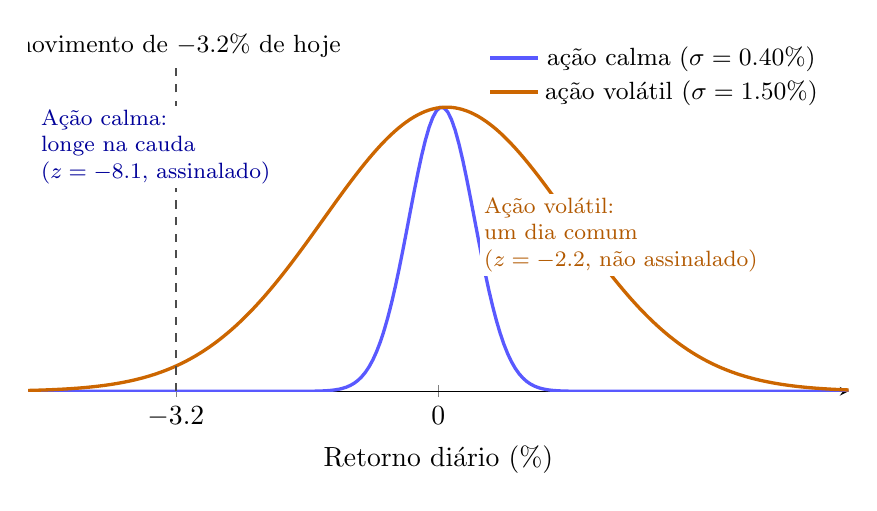
\begin{tikzpicture}
\begin{axis}[
  width=12cm, height=6.2cm,
  xlabel={Retorno diário (\%)}, xmin=-5, xmax=5,
  ymin=0, ymax=1.28, ytick=\empty,
  axis y line=none, axis x line=bottom,
  xtick={-3.2,0}, xticklabels={$-3.2$,$0$},
  every axis plot/.append style={very thick}, samples=220,
  legend style={at={(0.98,0.98)}, anchor=north east, draw=none, fill=none, font=\small},
]
  \addplot[blue!65, domain=-5:5]{exp(-(x-0.04)^2/(2*0.40^2))};
  \addlegendentry{ação calma ($\sigma=0.40\%$)}
  \addplot[orange!80!black, domain=-5:5]{exp(-(x-0.10)^2/(2*1.50^2))};
  \addlegendentry{ação volátil ($\sigma=1.50\%$)}
  \draw[dashed, black!70, thick] (axis cs:-3.2,0) -- (axis cs:-3.2,1.14);
  \node[anchor=south, font=\small] at (axis cs:-3.2,1.14) {movimento de $-3.2\%$ de hoje};
  \node[blue!60!black, anchor=west, align=left, font=\footnotesize, fill=white, inner sep=1.5pt]
       at (axis cs:-4.9,0.86) {Ação calma:\\ longe na cauda\\ ($z=-8.1$, assinalado)};
  \node[orange!70!black, anchor=west, align=left, font=\footnotesize, fill=white, inner sep=1.5pt]
       at (axis cs:0.5,0.55) {Ação volátil:\\ um dia comum\\ ($z=-2.2$, não assinalado)};
\end{axis}
\end{tikzpicture}
\caption[O mesmo movimento, duas ações diferentes]{Porque um limiar de percentagem fixa é rejeitado. Ambas
as ações caem $-3.2\%$ hoje (linha tracejada). Para a ação calma (distribuição estreita) esse movimento fica
bem na cauda ($z=-8.1$) e é assinalado; para a ação volátil (distribuição larga) o movimento idêntico fica
dentro do seu intervalo comum dia-a-dia ($z=-2.2$) e não é. O \emph{z}-score deslizante pergunta ``invulgar
\emph{para esta ação}?'', o que uma percentagem não consegue. Valores da
Tabela~\ref{tab:zscore_worked}.}
\label{fig:zscore_curves}
\end{figure}

\subsection{Recuperação Semântica e Medição de Impacto}
\label{sec:met_correlation}

\emph{Para que serve:} dada uma manchete nova, encontrar as manchetes passadas mais similares e mostrar o
que aconteceu aos seus preços. Este motor de correlação notícia--mercado é o coração do trabalho, e combina
duas técnicas. \emph{Recuperação:} cada manchete torna-se um embedding de frase com o Sentence-BERT
\autocite{reimers2019sbert}, escolhido (Secção~\ref{sec:sota_finnlp}) porque capta o significado mas produz
vetores diretamente comparáveis, pelo que os itens passados mais próximos são encontrados de forma barata
por similaridade do cosseno. \emph{Impacto:} para cada precedente, o retorno cumulativo é medido sobre
janelas pós-evento fixas ($+1$, $+3$ e $+5$ dias de negociação), à maneira de um estudo de evento
\autocite{fama1969adjustment, brown1985daily}. Tanto a métrica de similaridade como as janelas são escolhas
explícitas e documentadas, e em conjunto são a contribuição metodológica. O impacto é medido estritamente
após o evento, pelo que é um resultado, não uma previsão. O Algoritmo~\ref{alg:retrieval} enuncia o passo
recuperar-e-reutilizar (o núcleo de raciocínio baseado em casos da Secção~\ref{sec:sota_cbr}).

\begin{algorithm}[ht]
\caption{Recuperação de precedentes e reporte de impacto (gatilho de notícias).}
\label{alg:retrieval}
\begin{algorithmic}[1]
\Require manchete $h$; base de conhecimento $\mathcal{K}=\{(d_j,c_j,h_j,\mathbf{e}_j,\text{impacto}_j)\}$; vizinhos $k$; horizonte $\tau$
\Ensure top-$k$ precedentes com similaridade e impacto observado, e o seu impacto médio
\State $\mathbf{q} \gets \mathrm{embed}(h)$ \Comment{o mesmo modelo Sentence-BERT que a KB}
\For{cada caso $j \in \mathcal{K}$}
  \State $s_j \gets \cos(\mathbf{q}, \mathbf{e}_j)$ \Comment{cosseno sobre vetores L2-normalizados}
\EndFor
\State $S \gets$ índices dos $k$ maiores $s_j$
\State \Return $\{(d_j,c_j,h_j,s_j,\text{impacto}_j[\tau]) : j \in S\}$ e $\mathrm{mean}_{j\in S}\,\text{impacto}_j[\tau]$
\end{algorithmic}
\end{algorithm}

Dois detalhes do passo de embedding merecem ser explícitos, porque cada um responde a uma pergunta que
naturalmente se coloca. O primeiro é o que $\mathrm{embed}(h)$ de facto calcula. O Sentence-BERT é um
\emph{bi-encoder}: um transformer pré-treinado lê a manchete uma vez e produz um vetor contextual por token,
e o embedding de frase é a média desses vetores de token (mean pooling), escalado para comprimento
unitário:
\begin{equation}
\mathbf{e} \;=\; \frac{1}{n}\sum_{i=1}^{n} \mathbf{t}_i,
\qquad
\hat{\mathbf{e}} \;=\; \frac{\mathbf{e}}{\lVert \mathbf{e} \rVert_2},
\label{eq:pooling}
\end{equation}
onde $\mathbf{t}_1,\dots,\mathbf{t}_n$ são os vetores de token da camada final do transformer. O encoder em
produção (MiniLM) é um transformer destilado de seis camadas que produz embeddings de $384$ dimensões,
pequeno o suficiente para infraestrutura gratuita. O desenho bi-encoder é o que torna uma base de
conhecimento prática: cada caso guardado é embebido \emph{uma vez}, e uma manchete nova custa uma única
passagem para a frente mais comparações de vetores baratas. A alternativa cross-encoder, mais exata, que
relê a consulta e o candidato juntos, precisaria de uma passagem completa de transformer por par (consulta,
caso), o que à escala do Capítulo~\ref{chap:casestudies} significa dezenas de milhares de passagens por cada
manchete que chega. O segundo detalhe é a própria similaridade. Para embeddings $\mathbf{q}$ e $\mathbf{e}$,
\begin{equation}
\cos(\mathbf{q},\mathbf{e}) \;=\;
\frac{\mathbf{q}\cdot\mathbf{e}}{\lVert\mathbf{q}\rVert_2\,\lVert\mathbf{e}\rVert_2},
\qquad
\lVert \hat{\mathbf{q}} - \hat{\mathbf{e}} \rVert_2^2 \;=\; 2 - 2\cos(\hat{\mathbf{q}},\hat{\mathbf{e}}),
\label{eq:cosine}
\end{equation}
e a identidade da direita resolve a questão do ``porquê cosseno?'': em vetores de comprimento unitário o
cosseno iguala o produto interno, e a distância euclidiana é uma função monótona dele, pelo que as três
medidas de similaridade naturais induzem exatamente a mesma ordenação. A escolha do cosseno é, portanto,
canónica e não arbitrária; o que importa é a normalização L2, que impede que textos mais longos pareçam
artificialmente ``maiores'' do que os curtos.

O próprio impacto é lido de uma janela curta após o evento, como a Figura~\ref{fig:eventwindow} mostra. A
notícia pode chegar num dia não-negociável, pelo que o \emph{dia do evento} é o primeiro dia de negociação
em ou após ela; o retorno é então acumulado do fecho desse dia até ao fecho $+1$, $+3$ e $+5$ dias de
negociação depois. Ancorar no fecho, e olhar apenas para a frente, é o que mantém a medida livre de
lookahead: regista o que aconteceu \emph{depois} de o evento se tornar acionável, nunca antes.

\begin{figure}[ht]
\centering
\begin{tikzpicture}[font=\scriptsize, >={Stealth[length=2.2mm]}]
  % eixo do tempo
  \draw[->] (-2.0,0) -- (7.6,0) node[right, font=\tiny]{dias de negociação};
  \foreach \x in {0,1,3,5} {\draw (\x,0.1) -- (\x,-0.1);}
  % data da notícia (esquerda): traço tracejado + rótulo acima-esquerda, livre das setas
  \draw[dashed, black!55] (-1.3,0) -- (-1.3,0.5);
  \node[above, align=center, font=\tiny] at (-1.3,0.5) {notícia $d_i$\\(pode ser não-negociação)};
  % dia do evento
  \filldraw (0,0) circle (1.5pt);
  \node[below=9pt, align=center, font=\tiny] at (0,0) {dia do evento $e_i$\\(1.\textsuperscript{o} dia de negociação $\ge d_i$)};
  % marcas de horizonte (logo abaixo do eixo)
  \node[below=1pt, font=\tiny] at (1,0) {$+1$};
  \node[below=1pt, font=\tiny] at (3,0) {$+3$};
  \node[below=1pt, font=\tiny] at (5,0) {$+5$};
  % setas de retorno cumulativo, bem separadas, com um rótulo acima
  \draw[->, thick] (0,0.55) -- (1,0.55);
  \draw[->, thick] (0,0.95) -- (3,0.95);
  \draw[->, thick] (0,1.35) -- (5,1.35);
  \node[above, font=\tiny, text=black!70] at (2.5,1.45)
    {retorno cumulativo desde o fecho de $e_i$ \,($+1$, $+3$, $+5$ dias)};
\end{tikzpicture}
\caption[Janelas de impacto de estudo de evento]{Como o impacto é medido. A data da notícia $d_i$ pode cair
num dia não-negociável; o dia do evento $e_i$ é o primeiro dia de negociação em ou após ela. O retorno é
então acumulado para a frente a partir do fecho de $e_i$ ao longo de $+1$, $+3$ e $+5$ dias de negociação.
Apenas dias pós-evento são usados, pelo que nenhuma informação futura entra.}
\label{fig:eventwindow}
\end{figure}

Três escolhas fixam \emph{como} o impacto é medido, cada uma feita tanto pela transparência como pelo rigor:
\begin{itemize}
  \item \textbf{Horizontes.} Janelas curtas ($+1$, $+3$, $+5$ dias), padrão para estudos de evento diários
        \autocite{brown1985daily}; janelas mais longas deixam entrar movimentos não relacionados de todo o
        mercado.
  \item \textbf{Linha de base.} O retorno cumulativo \emph{bruto}, não um retorno anormal ajustado ao
        mercado, porque é diretamente observável e não precisa de um modelo de mercado estimado que um
        não-especialista não pudesse verificar. O custo, enunciado com clareza, é que um retorno bruto
        mistura a reação à notícia com qualquer movimento de todo o mercado nos mesmos dias (a ameaça de
        confundimento examinada no Capítulo~\ref{chap:casestudies}); o ajuste ao mercado é trabalho futuro.
  \item \textbf{Agregação.} O número de destaque é o impacto \emph{médio} sobre os precedentes recuperados,
        mas os precedentes individuais são sempre mostrados também, para que o investidor veja a dispersão,
        não apenas um número.
\end{itemize}

Vale a pena resolver aqui uma aparente inconsistência, porque duas partes do sistema medem o rescaldo de um
evento de forma diferente, e ambas estão certas para o seu trabalho. O impacto \emph{mostrado} de um
precedente usa o retorno bruto, como escolhido acima: é o que o investidor teria de facto experienciado, e
pode ser verificado contra qualquer gráfico de preços público. O \emph{rótulo} do modelo de triagem de
materialidade (Secção~\ref{sec:met_triage}) usa antes a diferença ajustada ao mercado
$\lvert r^{\mathrm{tkr}} - r^{\mathrm{mkt}} \rvert$, porque um alvo de treino tem de isolar o movimento
específico do ticker das oscilações de todo o mercado; caso contrário o modelo aprenderia a prever o índice
em vez das consequências da notícia. É a mesma maquinaria de estudo de evento a responder a duas perguntas
diferentes: ``o que aconteceu a esta ação?'' para a evidência mostrada a uma pessoa, e ``moveu-se esta ação
por razões próprias?'' para um rótulo que um modelo aprende.

Um exemplo trabalhado torna-o concreto. A Figura~\ref{fig:embedding_concept} dá a intuição: o embedding
coloca cada manchete num espaço onde temas semelhantes ficam próximos, pelo que uma consulta cai perto das
suas correspondências e longe de notícias não relacionadas.

\begin{figure}[ht]
\centering
\begin{tikzpicture}[font=\scriptsize, >={Stealth[length=2mm]}]
  \draw[rounded corners, draw=black!25] (-0.3,-0.4) rectangle (9.8,4.4);
  \node[font=\tiny, text=black!55] at (3.2,4.1) {espaço de embeddings (esquemático, 2-D para intuição)};
  % --- notícias não relacionadas (ocas), à esquerda, bem separadas ---
  \draw (0.9,3.4) circle (2.2pt) node[right=2pt, font=\tiny] {JPM perspetiva de taxas};
  \draw (0.9,2.2) circle (2.2pt) node[right=2pt, font=\tiny] {XOM movimento do petróleo};
  \draw (0.9,1.0) circle (2.2pt) node[right=2pt, font=\tiny] {TSLA recall};
  % --- cluster temático de IA (cheio = recuperado), à direita ---
  \coordinate (q)  at (5.35,3.10);
  \coordinate (p1) at (5.00,2.85);
  \coordinate (p2) at (5.60,2.60);
  \coordinate (p3) at (5.05,2.25);
  \draw[dashed, black!55] (5.30,2.65) ellipse (0.85 and 0.85);
  \node[star, star points=5, star point ratio=2.3, fill=black, inner sep=1.3pt] at (q) {};
  \fill (p1) circle (2.2pt);
  \fill (p2) circle (2.2pt);
  \fill (p3) circle (2.2pt);
  % rótulos à direita, com linhas guia finas (sem sobreposição)
  \node[font=\tiny, anchor=west] (lq) at (7.0,3.35) {consulta (manchete nova)};
  \node[font=\tiny, anchor=west] (l1) at (7.0,2.90) {NVDA: guidance de chips IA};
  \node[font=\tiny, anchor=west] (l2) at (7.0,2.45) {MSFT: procura de IA na nuvem};
  \node[font=\tiny, anchor=west] (l3) at (7.0,2.00) {NVDA: acelerador IA};
  \draw[black!45, line width=0.3pt] (q)  -- (lq.west);
  \draw[black!45, line width=0.3pt] (p1) -- (l1.west);
  \draw[black!45, line width=0.3pt] (p2) -- (l2.west);
  \draw[black!45, line width=0.3pt] (p3) -- (l3.west);
  \node[font=\tiny, text=black!55] at (5.30,1.55) {vizinhança top-$k$};
\end{tikzpicture}
\caption[Ilustração conceptual da recuperação semântica]{Ilustração conceptual da recuperação semântica.
Cada manchete torna-se um ponto num espaço de embeddings de dimensão elevada (desenhado em duas dimensões
apenas para intuição). Textos do mesmo tema ficam próximos, pelo que uma consulta (estrela) cai perto dos
seus precedentes semanticamente similares (cheios), que formam a vizinhança top-$k$, e longe de notícias não
relacionadas (ocas). A tabela seguinte torna isto concreto com números reais.}
\label{fig:embedding_concept}
\end{figure}

A Tabela~\ref{tab:retrieval_worked} corre o passo de ponta a ponta sobre a pequena base de conhecimento de
amostra que acompanha o sistema. Para a manter reprodutível sem descarregar um modelo, usa um encoder
transparente de sobreposição de palavras (o sistema em produção usa o Sentence-BERT, avaliado no
Capítulo~\ref{chap:casestudies}). Para a consulta \emph{``Nvidia demand surges on AI chip orders''}, os três
precedentes mais próximos são todos de tema IA e não todos da mesma empresa: um item de IA-na-nuvem da
Microsoft é recuperado a par de dois itens da Nvidia, mostrando a generalização \emph{cross-ticker} em que a
avaliação assenta. O seu impacto médio a $+5$ dias é $+6.5\%$, mostrado como evidência, com a ressalva
explícita de que regista o que se seguiu a notícias passadas comparáveis, não uma previsão.

\begin{table}[ht]
\caption{Exemplo trabalhado de recuperação sobre a base de conhecimento de amostra incluída. Consulta:
\emph{``Nvidia demand surges on AI chip orders''}; as similaridades e impactos são reais e reprodutíveis.}
\label{tab:retrieval_worked}
\centering
\begin{tabular}{c c c p{0.38\textwidth}}
\toprule
\tabhead{Similaridade} & \tabhead{Impacto +5 dias} & \tabhead{Ticker / data} & \tabhead{Manchete recuperada (excerto)} \\
\midrule
$0.60$ & $+3.5\%$  & NVDA, 2023-05-25 & Nvidia guidance surges on soaring demand for AI data-centre chips \\
$0.38$ & $+10.9\%$ & MSFT, 2023-04-25 & Microsoft cloud growth accelerates on AI demand \\
$0.38$ & $+4.9\%$  & NVDA, 2023-06-13 & Nvidia unveils new AI accelerator to extend data-centre lead \\
\midrule
\multicolumn{4}{l}{\textbf{Impacto médio a $+5$ dias sobre os precedentes recuperados: $+6.5\%$}} \\
\bottomrule
\end{tabular}

\smallskip
{\footnotesize\emph{Nota:} a média é calculada a partir dos impactos não arredondados, pelo que não tem de
igualar a média dos valores arredondados mostrados.}
\end{table}

\subsection{Triagem de Materialidade: um Modelo de Severidade Treinado}
\label{sec:met_triage}

\emph{Para que serve:} ordenar o fluxo de notícias que chega, para que a atenção limitada do utilizador vá
para as manchetes com maior probabilidade de importar (Secção~\ref{sec:sota_triage}), respondendo à
\gls{RQ}4.

A unidade é um triplo (manchete, ticker, dia do evento), onde o dia do evento $d$ é o primeiro dia de
negociação em ou após a data da notícia, a mesma regra de alinhamento que a base de conhecimento usa. O
rótulo faz uma pergunta livre de direção por construção: seguiu-se um movimento anormal de tamanho invulgar?
Formalmente, o exemplo é \emph{material} quando
$|r^{\mathrm{tkr}}_{(d,\,d+h]} - r^{\mathrm{mkt}}_{(d,\,d+h]}| \ge \tau$. A quantidade dentro do valor
absoluto é o retorno do ticker sobre os $h$ dias de negociação após o evento menos o do mercado (um proxy de
índice): o resultado ajustado ao mercado da Secção~\ref{sec:sota_eventstudy}. A definição primária é
$\tau = 2\%$ a $h = 3$; uma grelha de sensibilidade sobre $\tau \in \{1.5\%, 2\%, 3\%\}$ e
$h \in \{1, 3, 5\}$ é reportada para que a conclusão não dependa de um só limiar. Os rótulos são produzidos
pelo próprio código de estudo de evento do sistema; não há anotação manual envolvida.

As features respeitam uma convenção temporal estrita, todas calculáveis no fecho do dia $d$, antes de a
janela do rótulo abrir: a volatilidade pré-evento (desvio-padrão dos vinte log-retornos diários que terminam
no dia \emph{anterior} ao evento), o momentum de cinco dias até ao mesmo ponto, o próprio retorno do dia do
evento (conhecido no fecho de $d$), o comprimento da manchete, um indicador de setor, e o embedding de frase
da manchete. Um teste unitário impõe a convenção ao mutar preços \emph{depois} da janela do evento e
verificar que nenhuma feature muda enquanto o rótulo muda.

A Tabela~\ref{tab:met_features} torna essas colunas concretas: lista cada feature, o que é, e o seu valor
real para o exemplo trabalhado da Figura~\ref{fig:data_journey} (Nvidia, 10~de~maio~de~2018), juntamente com
o rótulo-alvo. Estes são exatamente os dados sobre os quais as métricas são calculadas.

\begin{table}[ht]
\caption[As colunas de features da triagem, com valores reais]{As colunas que o modelo de triagem lê, com
os seus valores reais para um exemplo (Nvidia, 10~de~maio~de~2018). As linhas 1--6 são as features; a última
linha é o alvo supervisionado. As colunas de contexto (1--5) alimentam as regressões logísticas e o ensemble
com gradient boosting, pontuadas por PR-AUC e precisão@5/dia; o embedding (6) também alimenta a recuperação
de precedentes, pontuada por precisão@$k$. Cada feature é calculável no fecho do dia $d$, antes de a janela
do rótulo abrir.}
\label{tab:met_features}
\centering
\small
\begin{tabular}{l p{6.4cm} l}
\toprule
\tabhead{Atributo} & \tabhead{O que é} & \tabhead{Valor de exemplo} \\
\midrule
Volatilidade pré-evento & desvio-padrão dos 20 log-retornos diários que terminam em $d{-}1$ & $0.021$ \\
Momentum de cinco dias & log-retorno cumulativo até $d{-}1$ & $+0.122$ \\
Retorno do dia do evento & log-retorno de $d$, conhecido no seu fecho & $+0.017$ \\
Comprimento da manchete & número de caracteres na manchete & $55$ \\
Setor & indicador de setor one-hot & tech \\
Embedding da manchete & vetor Sentence-BERT de $384$ dimensões & $[-0.005, 0.004, \dots]$ \\
\midrule
Materialidade \emph{(alvo)} & $|$retorno anormal vs SPY sobre $(d,d{+}3]| \ge 2\%$ & $1$ (material) \\
\bottomrule
\end{tabular}
\end{table}

As famílias de modelos abrangem o compromisso interpretabilidade--capacidade da
Secção~\ref{sec:sota_triage}: um chão de alertar-sempre, uma regressão logística só-volatilidade (a regra
ingénua forte que qualquer revisor perguntaria), regressões logísticas só sobre features de contexto, só
sobre features de texto, e sobre ambas em conjunto (o principal modelo interpretável), e um ensemble com
gradient boosting \autocite{friedman2001gbm} como teto de capacidade.

O membro interpretável dessa família merece a sua matemática por inteiro, porque as explicações em produção
decompõem-na termo a termo. Com features padronizadas $\tilde{x}_1,\dots,\tilde{x}_m$, a regressão logística
pontua um exemplo como
\begin{equation}
u \;=\; b_0 + \sum_{j=1}^{m} w_j\,\tilde{x}_j,
\qquad
p_{\text{raw}} \;=\; \sigma(u) \;=\; \frac{1}{1+e^{-u}},
\label{eq:logistic}
\end{equation}
pelo que cada produto $w_j\tilde{x}_j$ é uma contribuição aditiva \emph{exata} para os log-odds $u$: sem
modelo substituto e sem aproximação, a propriedade que torna a linha do ``porquê'' do alerta fiel por
construção. Como uma pontuação discriminativa não é automaticamente uma probabilidade honesta, uma
calibração de Platt é ajustada apenas sobre o bloco de validação,
\begin{equation}
p \;=\; \sigma\!\big(a\,p_{\text{raw}} + c\big),
\label{eq:platt}
\end{equation}
com apenas dois escalares $(a, c)$. A forma paramétrica é uma escolha deliberada face à alternativa
não-paramétrica, a regressão isotónica: uma sigmoide de dois parâmetros não pode sobreajustar um bloco de
validação modesto, ao passo que a regressão isotónica precisa de substancialmente mais dados de calibração
antes de a sua flexibilidade extra compensar \autocite{niculescu2005calibration}. Uma comparação isotónica
sobre o corpus completo é notada como trabalho futuro em vez de assumida num sentido ou noutro.

A Tabela~\ref{tab:triage_worked} torna todo o cálculo concreto ao decompor uma decisão de produção
\emph{real}: uma manchete da Meta enviada ao canal público de alertas a 12 de julho de 2026, pontuada pelo
bundle só-contexto em produção. Ler a tabela de cima a baixo é ler as Equações~\eqref{eq:logistic} e
\eqref{eq:platt} com números no lugar: a volatilidade recente elevada e o indicador de setor empurram os
log-odds para cima, os termos quase-zero mal os movem, a soma dá $u = +0.699$, a sigmoide transforma-o em
$p_{\text{raw}} = 0.668$, e o mapa de Platt (valores ajustados $a = 3.700$, $c = -2.313$) produz o $p =
0.539$ calibrado, que ultrapassa a porta de implantação de $0.5$. A mensagem efetivamente entregue ao canal
nesse dia dizia \emph{``Risk estimate (learned triage): 54\% \dots raised by recent volatility (20d) and
sector''}: a decomposição reproduz o número de produção e os seus fatores dominantes exatamente. Para as
explicações, as dimensões do embedding (quando a variante de texto é usada) são agrupadas num único termo
``conteúdo da manchete'' para que a mensagem se mantenha legível, e cada pontuação é entregue com a cláusula
fixa \emph{``triage evidence, not a forecast''}.

\begin{table}[ht]
\caption[Exemplo de triagem trabalhado: um alerta de produção real decomposto]{Exemplo de triagem
trabalhado: o modelo só-contexto em produção a pontuar um alerta real (META, 12 de julho de 2026,
\emph{``Mark Zuckerberg Said Meta's AI Bets `Haven't Come to Fruition Yet' as Shares Fell 5\%''}). As
contribuições são os termos aditivos exatos $w_j\tilde{x}_j$ da Equação~\eqref{eq:logistic}; a decomposição é
regenerada deterministicamente a partir dos inputs congelados.}
\label{tab:triage_worked}
\centering
\begin{tabular}{l r}
\toprule
\tabhead{Termo} & \tabhead{Contribuição para os log-odds} \\
\midrule
Interceção $b_0$ & $-0.025$ \\
Volatilidade recente (20\,d) & $+0.409$ \\
Indicador de setor & $+0.303$ \\
Retorno do dia do evento & $+0.010$ \\
Comprimento da manchete & $+0.002$ \\
Momentum recente (5\,d) & $+0.000$ \\
\midrule
Log-odds $u$ (soma) & $\mathbf{+0.699}$ \\
Probabilidade crua $\sigma(u)$ & $0.668$ \\
$p$ calibrado $= \sigma(3.700\,p_{\text{raw}} - 2.313)$ & $\mathbf{0.539}$ \\
Porta de implantação $p \ge 0.5$ & passou (alerta enviado) \\
\bottomrule
\end{tabular}
\end{table}

A implantação é deliberadamente conservadora. A pontuação entra na pipeline de alertas desligada por
defeito, atrás de uma porta de configuração; a variante em produção usa apenas features de contexto, pelo
que corre na stack de software leve, e o texto do alerta nomeia a variante usada. Uma vez ao vivo, cada
decisão de triagem é registada, e um passo de pós-validação rotula depois cada decisão maturada com o que
efetivamente aconteceu, usando a mesma regra de rótulo, produzindo monitorização de precisão e calibração ao
vivo e dados de treino frescos. Isto é aprendizagem contínua com rótulos atrasados, não aprendizagem por
reforço: não há ciclo de feedback ação--ambiente, porque os alertas do sistema não movem o mercado.

\subsection{Técnicas de Explicação}
\label{sec:met_xai}

\emph{Para que serve:} transformar os objetos calculados numa mensagem que o investidor possa verificar. A
explicação é procurada por desenho transparente (Secção~\ref{sec:sota_xai})
\autocite{rudin2019stop, arrieta2020xai}. Cada alerta é montado a partir de três ingredientes
transparentes: a regra que disparou (o $z$-score com a sua janela e limiar); os precedentes recuperados com
o seu impacto observado; e, opcionalmente, a atribuição de features sobre o detetor com o SHAP
\autocite{lundberg2017shap}. O sentimento financeiro de um modelo de domínio \autocite{araci2019finbert} é
um enriquecimento opcional, usado apenas se acrescentar valor defensável. Como cada alerta é composto
diretamente a partir destes objetos, a explicação é fiel ao cálculo por construção, uma propriedade testada
no Capítulo~\ref{chap:casestudies}.

\section{Ferramentas e Frameworks}
\label{sec:met_tools}

O sistema é construído sobre o ecossistema científico open-source de Python: bibliotecas maduras e gratuitas
para computação numérica, acesso a dados de mercado, embeddings de frase e figuras. Isto encaixa na
restrição de recursos gratuitos e na reprodutibilidade, já que dependências fixadas e sementes fixas
permitem recriar o ambiente e os resultados noutro lugar. O ambiente de reprodução e as saídas de avaliação
estão reunidos no Apêndice~\ref{app:reproducibility}, para que este capítulo se possa focar nos próprios
\emph{métodos}.

\section{IA Responsável e Ética}
\label{sec:met_ethics}

O trabalho está vinculado a vários compromissos de IA responsável que decorrem diretamente do seu propósito
e do seu público. \textbf{Sem aconselhamento e sem previsão:} o sistema não faz previsão de preços nem
recomendação de negociação; traz à superfície resultados passados observados como evidência e declara-o
explicitamente em cada alerta, para que o investidor seja informado e não instruído. \textbf{Transparência:}
cada alerta expõe a sua cadeia de raciocínio completa, em consonância com os princípios de explicabilidade
do Capítulo~\ref{chap:sota}, para que um utilizador possa verificar em vez de meramente confiar na saída.
\textbf{Evidência honesta:} apenas os resultados que podem ser reproduzidos e explicados são reportados, e
nenhum dado, métrica ou citação é fabricado. \textbf{Gestão de dados:} todas as fontes são usadas dentro das
suas camadas gratuitas e licenças, o conjunto de dados FNSPID é atribuído como a sua licença Creative
Commons exige \autocite{dong2024fnspid}, o texto de notícias de terceiros não é republicado, e nenhum dado
pessoal é processado. \textbf{Segurança:} as credenciais nunca são guardadas em ficheiros versionados. Por
fim, o sistema é posicionado como um auxílio ao apoio à decisão para um investidor não-profissional, não
como substituto de aconselhamento profissional, uma limitação enunciada com clareza.

\section{Metodologia de Avaliação}
\label{sec:met_evaluation}

\emph{Como é o sistema julgado?} Por um plano fixado antes de qualquer experiência correr, para que a
métrica não possa ser escolhida a posteriori para lisonjear o resultado, um pré-registo em pequena escala.
Os resultados estão no Capítulo~\ref{chap:casestudies}; aqui está o protocolo que seguem.

\subsection{Métrica de recuperação e relevância}
\label{sec:met_eval_retrieval}

A recuperação é avaliada como uma tarefa de recuperação de informação (Secção~\ref{sec:sota_ir}) com
precisão@$k$, a fração dos $k$ primeiros precedentes que são relevantes. Escrevendo $Q$ para o conjunto de
manchetes de consulta e $R_k(q)$ para os $k$ primeiros itens devolvidos para a consulta $q$,
\begin{equation}
\text{precisão@}k = \frac{1}{|Q|}\sum_{q\in Q}\frac{1}{k}\sum_{d\in R_k(q)} \mathrm{rel}(q,d),
\qquad
\mathrm{rel}(q,d)=\mathbf{1}\big[\,\mathrm{setor}(d)=\mathrm{setor}(q)\,\big].
\label{eq:precatk}
\end{equation}
A relevância é aproximada por \emph{concordância de setor}: um precedente conta como relevante se a sua
empresa está no setor da consulta. Este é um substituto automático para ``análogo'', usado porque não existe
conjunto rotulado; os seus limites são enunciados com os resultados. Duas escolhas tornam a métrica
exigente, não lisonjeira. Primeiro, uma restrição \emph{cross-ticker} estrita descarta cada precedente que
partilha o ticker da consulta, pelo que o sistema não pode vencer ao emparelhar uma empresa com as suas
próprias notícias passadas; tem de generalizar \emph{entre} empresas de um setor. Segundo, $k$ é pequeno (o
número de destaque usa $k=5$), refletindo que um alerta mostra apenas alguns precedentes.

\subsection{Linhas de base}
\label{sec:met_eval_baselines}

Um único número significa pouco isolado, pelo que a recuperação semântica é comparada contra três linhas de
base, cada uma a controlar por uma explicação rival. \textbf{Aleatória} tira $k$ precedentes ao acaso; a sua
precisão é a taxa-base do setor, o chão sem-perícia. \textbf{Recência} devolve os itens mais recentes,
testando se simplesmente trazer notícias frescas à superfície faria igualmente bem. \textbf{Lexical} ordena
por sobreposição de palavras sob o mesmo cosseno, pelo que a diferença para o modelo de embedding isola o
valor do \emph{significado} sobre as palavras de superfície. Cada comparação é repetida sobre cinco sementes
aleatórias (média com desvio-padrão), e duas variantes do Sentence-BERT são tentadas, para que o resultado
reflita a recuperação semântica em geral, não uma tiragem de sorte ou um modelo.

\subsection{Protocolo de deteção de anomalias}
\label{sec:met_eval_anomaly}

O detetor de anomalias é julgado sobretudo por um argumento que não precisa de \emph{rótulo}: um bom detetor
universal deve disparar a uma taxa comparável em instrumentos de volatilidade muito diferente, ao passo que
uma regra cega à volatilidade não consegue. A consistência é, portanto, medida como a amplitude (máximo
menos mínimo) das taxas de disparo por ticker: quanto menor a amplitude, mais uniforme o detetor. Só
secundariamente é o detetor pontuado contra um proxy explícito de \emph{movimentos extremos} (um movimento
diário no ou além do percentil $99$ dos próprios retornos desse ticker), via precisão, recall e $F_1$; como
este proxy é ele próprio relativo à volatilidade, é tratado como evidência de apoio e não primária. Uma
ablação sobre o comprimento da janela de estimação completa o quadro ao expor a sensibilidade do detetor ao
seu único parâmetro principal. Por fim, a regra transparente é desafiada por um detetor \emph{aprendido} em
igualdade de circunstâncias: uma Isolation Forest \autocite{liu2008isolation} treinada causalmente sobre a
mesma informação (o retorno de cada dia e a volatilidade dos vinte dias anteriores, ajustada apenas sobre um
segmento passado inicial) é pontuada sobre a mesma região de avaliação, pelo que a escolha de uma regra
estatística em vez de uma aprendida é testada, não assumida. Duas extensões endurecem ainda mais essa
comparação. O Local Outlier Factor \autocite{breunig2000lof}, citado no Capítulo~\ref{chap:sota} como a
alternativa baseada em densidade, é avaliado sob o protocolo causal idêntico, pelo que a regra estatística
enfrenta \emph{dois} detetores aprendidos em vez de um. E a estimativa de volatilidade deslizante é desafiada
por uma variante ponderada exponencialmente (estilo RiskMetrics, $\lambda = 0.94$), o primeiro passo
empírico rumo à família GARCH da Secção~\ref{sec:sota_anomaly}, para que a pergunta natural ``porquê não
GARCH?'' receba evidência e não opinião.

\subsection{Protocolo de triagem}
\label{sec:met_eval_triage}

O modelo de materialidade da Secção~\ref{sec:met_triage} é avaliado sob um protocolo temporal estrito. Os
exemplos são divididos em blocos de treino, validação e teste cronologicamente, por \emph{dia de evento
único} (70/15/15), para que todas as manchetes de um dia caiam no mesmo bloco, e um embargo de vários dias
de negociação é removido após cada fronteira para que nenhuma janela de rótulo possa cavalgar dois blocos. A
calibração é ajustada apenas sobre o bloco de validação; o bloco de teste é tocado uma vez, para reportar. A
métrica primária é a área sob a curva de precisão-recall, cujo chão é a prevalência do teste (uma estratégia
de alertar-sempre); a área sob a curva ROC e o Brier score completam o quadro, e uma métrica em forma de
produto, a precisão dentro de um orçamento de $N$ alertas por dia, mede o que o utilizador de facto
experiencia. As métricas em si são padrão mas vale a pena fixá-las com precisão. Varrer um limiar $s$ sobre
as pontuações traça $\big(\mathrm{recall}(s), \mathrm{precisão}(s)\big)$; a PR-AUC é a área sob essa curva, e
um scorer sem perícia ganha exatamente a prevalência $\pi$, que ancora cada comparação. A ROC-AUC é a
probabilidade de um positivo aleatório superar um negativo aleatório; é reportada por completude mas não
usada como primária, porque premeia ordenar os abundantes negativos fáceis e por isso lisonjeia um modelo de
triagem cujo utilizador só vê o topo da ordenação. A calibração é medida pelo Brier score,
\begin{equation}
\mathrm{Brier} \;=\; \frac{1}{N}\sum_{i=1}^{N}\big(p_i - y_i\big)^2 ,
\label{eq:brier}
\end{equation}
a diferença quadrática média entre a probabilidade declarada $p_i$ e o resultado $y_i \in \{0,1\}$: é baixa
apenas quando as probabilidades podem ser tomadas pelo seu valor facial, que é exatamente o que um
utilizador a ler ``$57\%$'' merece. A comparação decisiva é contra a regressão logística só-volatilidade: o
modelo aprendido é considerado útil apenas onde bate essa linha de base, e as ablações de features (só
contexto, só texto, ambas) atribuem qualquer ganho à sua fonte. A sensibilidade sobre a grelha de rótulos
$\tau \times h$ é reportada a par. Duas garantias adicionais são pré-comprometidas. O treino é determinístico
dada a semente, e re-corrê-lo reproduz os artefactos guardados exatamente. E o resultado é reportado seja
qual for o sentido em que cai: se o modelo treinado não bater a linha de base da volatilidade num dado
corpus, esse achado fica tal como enunciado.

\subsection{Explicação, âmbito e garantias de rigor}
\label{sec:met_eval_rigour}

O motor de explicação é avaliado pela \emph{fidelidade}: se o texto do alerta reflete o cálculo real do
sistema. Isto verifica-se por construção, porque cada alerta é composto diretamente a partir dos objetos
calculados. A sua \emph{utilidade} para um investidor real é uma questão separada, que precisaria de um
estudo humano ainda não conduzido, e é reportada como uma limitação e não como uma afirmação. Como o sistema
não faz previsão de preços nem negociação, as métricas baseadas em lucro estão fora de âmbito por desenho,
não omitidas por conveniência. Sustentando cada experiência estão três garantias. Primeira, \textbf{sem
lookahead}: qualquer feature calculada num instante usa apenas informação disponível nesse instante ou
antes, e o impacto histórico usa apenas janelas pós-evento. Segunda, \textbf{reprodutibilidade}: as sementes
aleatórias são fixas, as dependências são fixadas, e cada figura de dados e de resultados é produzida por um
script versionado. Terceira, \textbf{honestidade}: os resultados são reportados com as suas ressalvas, e
achados modestos mas genuínos são preferidos a inflacionados.

\section{Conclusões do Capítulo}
\label{sec:met_summary}

Este capítulo fixou o método: simplicidade defensável e entrega incremental; uma arquitetura de dados de
duas camadas numa data card reprodutível; as técnicas de deteção, recuperação, impacto e explicação, cada
uma introduzida pelo seu propósito; e uma avaliação fixada à partida. O próximo capítulo reúne estas no
InvestiGator.
